\section{Überarbeitung der Android Application}

	\subsection{Motivation und Ziel}\label{motiv}
	Da die bisher vorhandene native Android Anwendung mit dem Hauptaugenmerk auf das Prototyping entwickelt wurde und aus diesem Grund kein spezielles Design sein eigen nennen kann, haben wir uns dazu entschieden, die Application von ihrem Status als Prototyp weg weiter zu entwickeln.\\
	Das Hauptaugenmerk sollte auf einer einfachen und verständlichen Bedienung sowie der Erstellung eines individuellen Designs liegen. Bestand die vorhandene App bisher nur aus einer Activity in welcher alle Interaktionen mit dem System ausgeführt wurden, so wurde die neue Anwendung etwas entzerrt und auf zwei Activities aufgeteilt. Auf diese beiden wurde die Nutzerführung und das gesamte Bedienkonzept angepasst und überarbeitet.\\

	\begin{figure}[htbp]
		\centering
		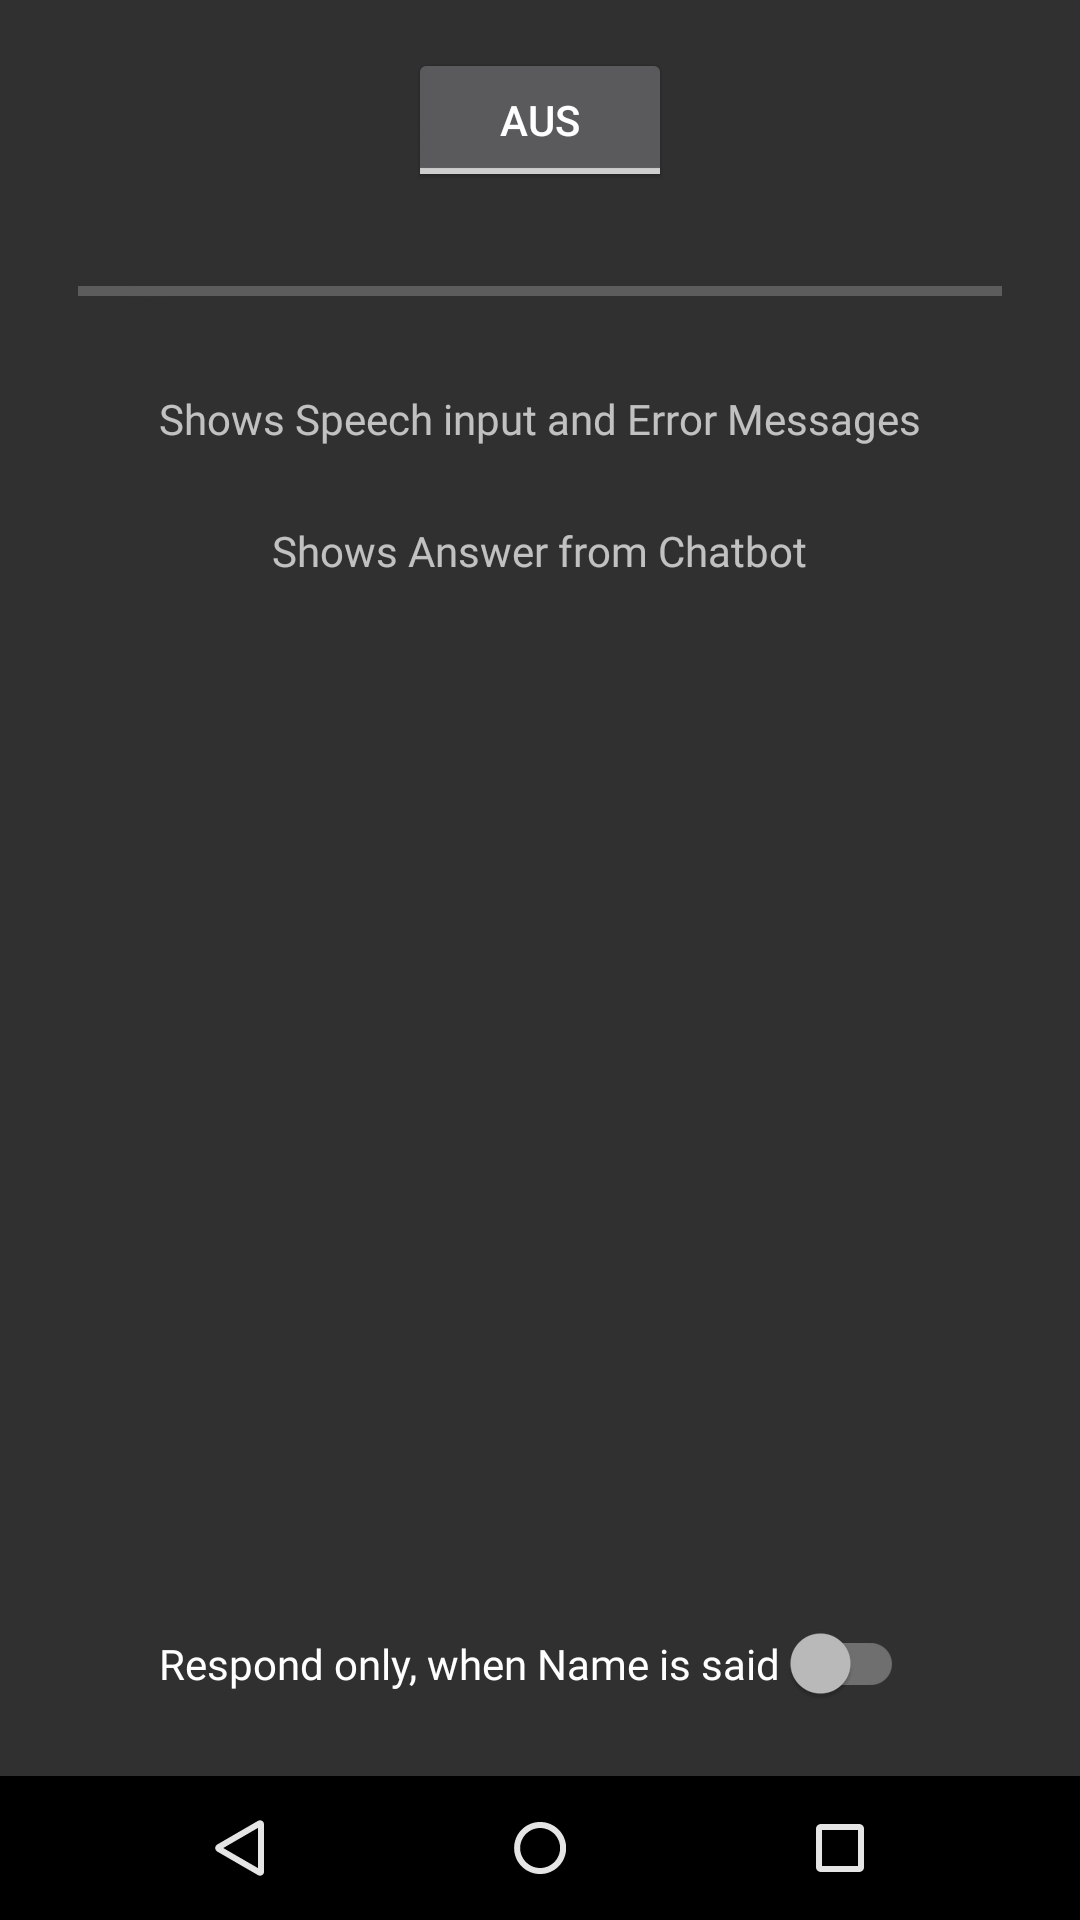
\includegraphics[height=0.8\textwidth]{dh/graphics/hablame-old.png}
		\caption{UI der bisherigen Android App}
		\label{fig:hablame-old}
	\end{figure} \leavevmode \\

	\subsection{Aufbau}\label{aufbau}

	Wie unter \ref{motiv} "Motivation und Ziel"' auf S.\pageref{motiv} bereits erwähnt, sollte die Anwendung auf zwei Activities aufgeteilt werden. Desweiteren beinhaltet sie eine Klasse für den zur Spracherkennung notwendigen Service - "RecognitionService.java" - und eine Klasse in welcher die möglichen Fehler des Service beschrieben werden, ErrorDescription.java. \\
	
	Bestandteile:
	\begin{itemize}\itemsep0pt
		\item MainActivity.java
		\item ConversationActivity.java
		\item RecognitionService.java
		\item ErrorDescription.java
	\end{itemize}
	
		\subsubsection{MainActivity}\label{mainact}
		Die MainActivity wird bei Programmstart automatisch geöffnet und bildet somit die Landing-Page. Sie besteht aus 3 grundlegenden Bereichen, nämlich dem Header, dem Body und dem Footer. Im Header sind die Schriftzüge "Háblame"' sowie "Das sprechende Faultier"' zu lesen.\\
		Der Body beinhaltet zum einen das Logo und ein editierbares Textfeld welches Nutzereingaben entgegennimmt, in diesem Fall speziell den Nutzernamen. Der Body bietet somit im Gegensatz zum Header eine Interaktionsmöglichkeit für den Nutzer.\\
		Der Footer besteht einzig aus einem Button welcher die komplette Displaybreite nutzt und bei einer onClick-Aktion auf die ConversationActivity weiterleitet. Diese Weiterleitung jedoch funktioniert nur wenn durch den Benutzer ein Username vergeben wurde, ansonsten wird eine Meldung auf dem Bildschirm ausgegeben, das kein Benutzername eingetragen ist. \\

		\subsubsection{ConversationActivity}\label{convact}
		
		Die ConversationActivity wird durch einen Intent in der MainActivity aufgerufen. Sie besteht ebenfalls aus Header Body und Footer. Änderungen gegenüber der MainActivity sind die Konversationsansicht im Body sowie eine andere Funktion des Buttons im Footer. Dieser bringt den Nutzer zurück in die MainActivity.\\
		Nach aufrufen der ConversationActivity wird der RecognitionService gestartet und der in der MainActivity zuvor eingegebene Nutzername in die Konversationsansicht übernommen.\\
				
		\subsubsection{RecognitionService und ErrorDescription}\label{recogError}
		Der RecognitionService welcher zur Erkennung der Sprache des Nutzers und deren Umsetzung in Text dient - und vice versa, wurde rein funktionell fast im Original übernommen. Einzig die Einbindung des alten Webservice wurde durch die Entwicklung und den Einsatz der Service-API-Library obsolet.\\
		Die Klasse ErrorDescription dient lediglich dem RecognitionService dazu um im Fehlerfall eine detaillierte Fehlerbeschreibung an den Nutzer zurück zu liefern.

	\subsection{Funktionsweise}\label{funktion}
	
	\begin{figure}[htbp]
		\centering
		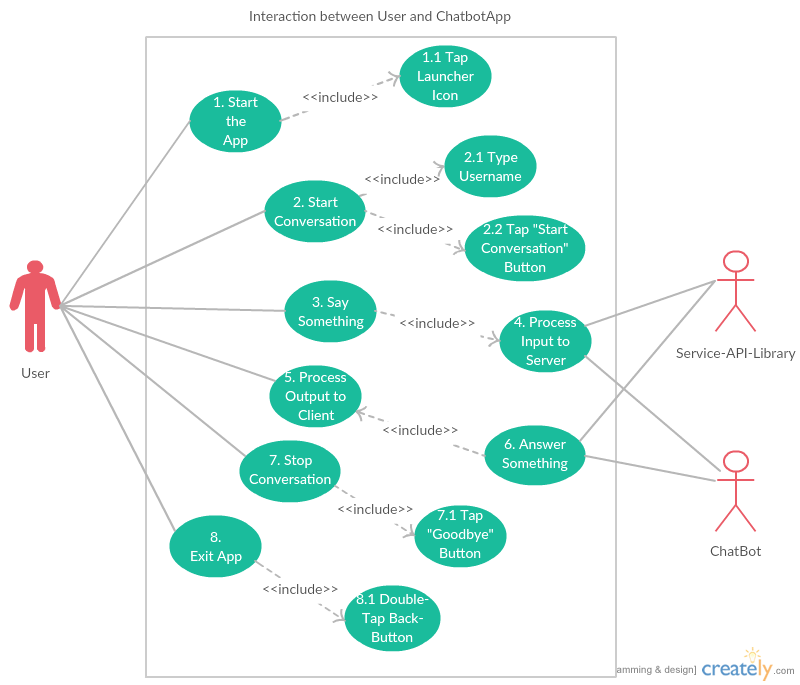
\includegraphics[height=0.9\textwidth]{dh/graphics/UseCaseChatbotApp.png}
		\caption{Use Case Diagramm zur Nutzung der App}
		\label{fig:usecaseapp}
	\end{figure} \leavevmode \\
	
	\subsection{Designanmerkungen}\label{design}
	
	Kritikpunkte bei der Erstellung:
	\begin{itemize}\itemsep0pt
	\item Entzerrung der Nutzerführung
	\item Erstellung eines Logos
	\item Wiedererkennungswert schaffen
	\item Individualität\\
	\end{itemize}
	Das UI wurde so erstellt um eine möglichst hohe Darstellbarkeit zu gewährleisten und der Fragmentierung auf Android bei zu kommen. So wurden bis auf das Logo selbst alle Elemente mit Android eigenen Bordmitteln umgesetzt um responsive zu bleiben. Das Logo wurde aus selbigem Grund in allen Auflösungen von ldpi bis xxhdpi umgesetzt.\\
	Eingesetzt wurde die, für kommerzielle sowie private Zwecke, frei nutzbare Schriftart Logobloqo2.ttf von seextwood\footnote{\label{foot:1}http://www.dafont.com/de/logobloqo2.font}. Sowie die Grafik "Cartellone con bradipo"' von bradisoft\footnote{\label{foot:2}https://de.fotolia.com/id/60029011}, die auf http://www.fotolia.de erworbene Vektorgrafik ist lizenzfrei und zeitlich sowie räumlich ohne Beschränkung nutzbar.\\
	
	\subsubsection{Farben}\label{farben}
		
		Alle verwendeten Farben sind dem Google Design Guide entnommen\footnote{\label{foot:3}https://www.google.com/design/spec/style/color.html\#color-color-palette}.\\
		
	MainActivity:
		\begin{itemize}\itemsep0pt
			\item Red 500
			\item Red 50
			\item Grey 400
		\end{itemize}
	
	ConversationActivity:
		\begin{itemize}\itemsep0pt
			\item Green 500
			\item Red 50
			\item Grey 400\\
		\end{itemize}
	Um die gestartete Konversation zu verdeutlichen, wurde für die ConversationActivity bewusst eine andere Hauptfarbe gewählt.
	
	\begin{figure}[htbp]
		\centering
		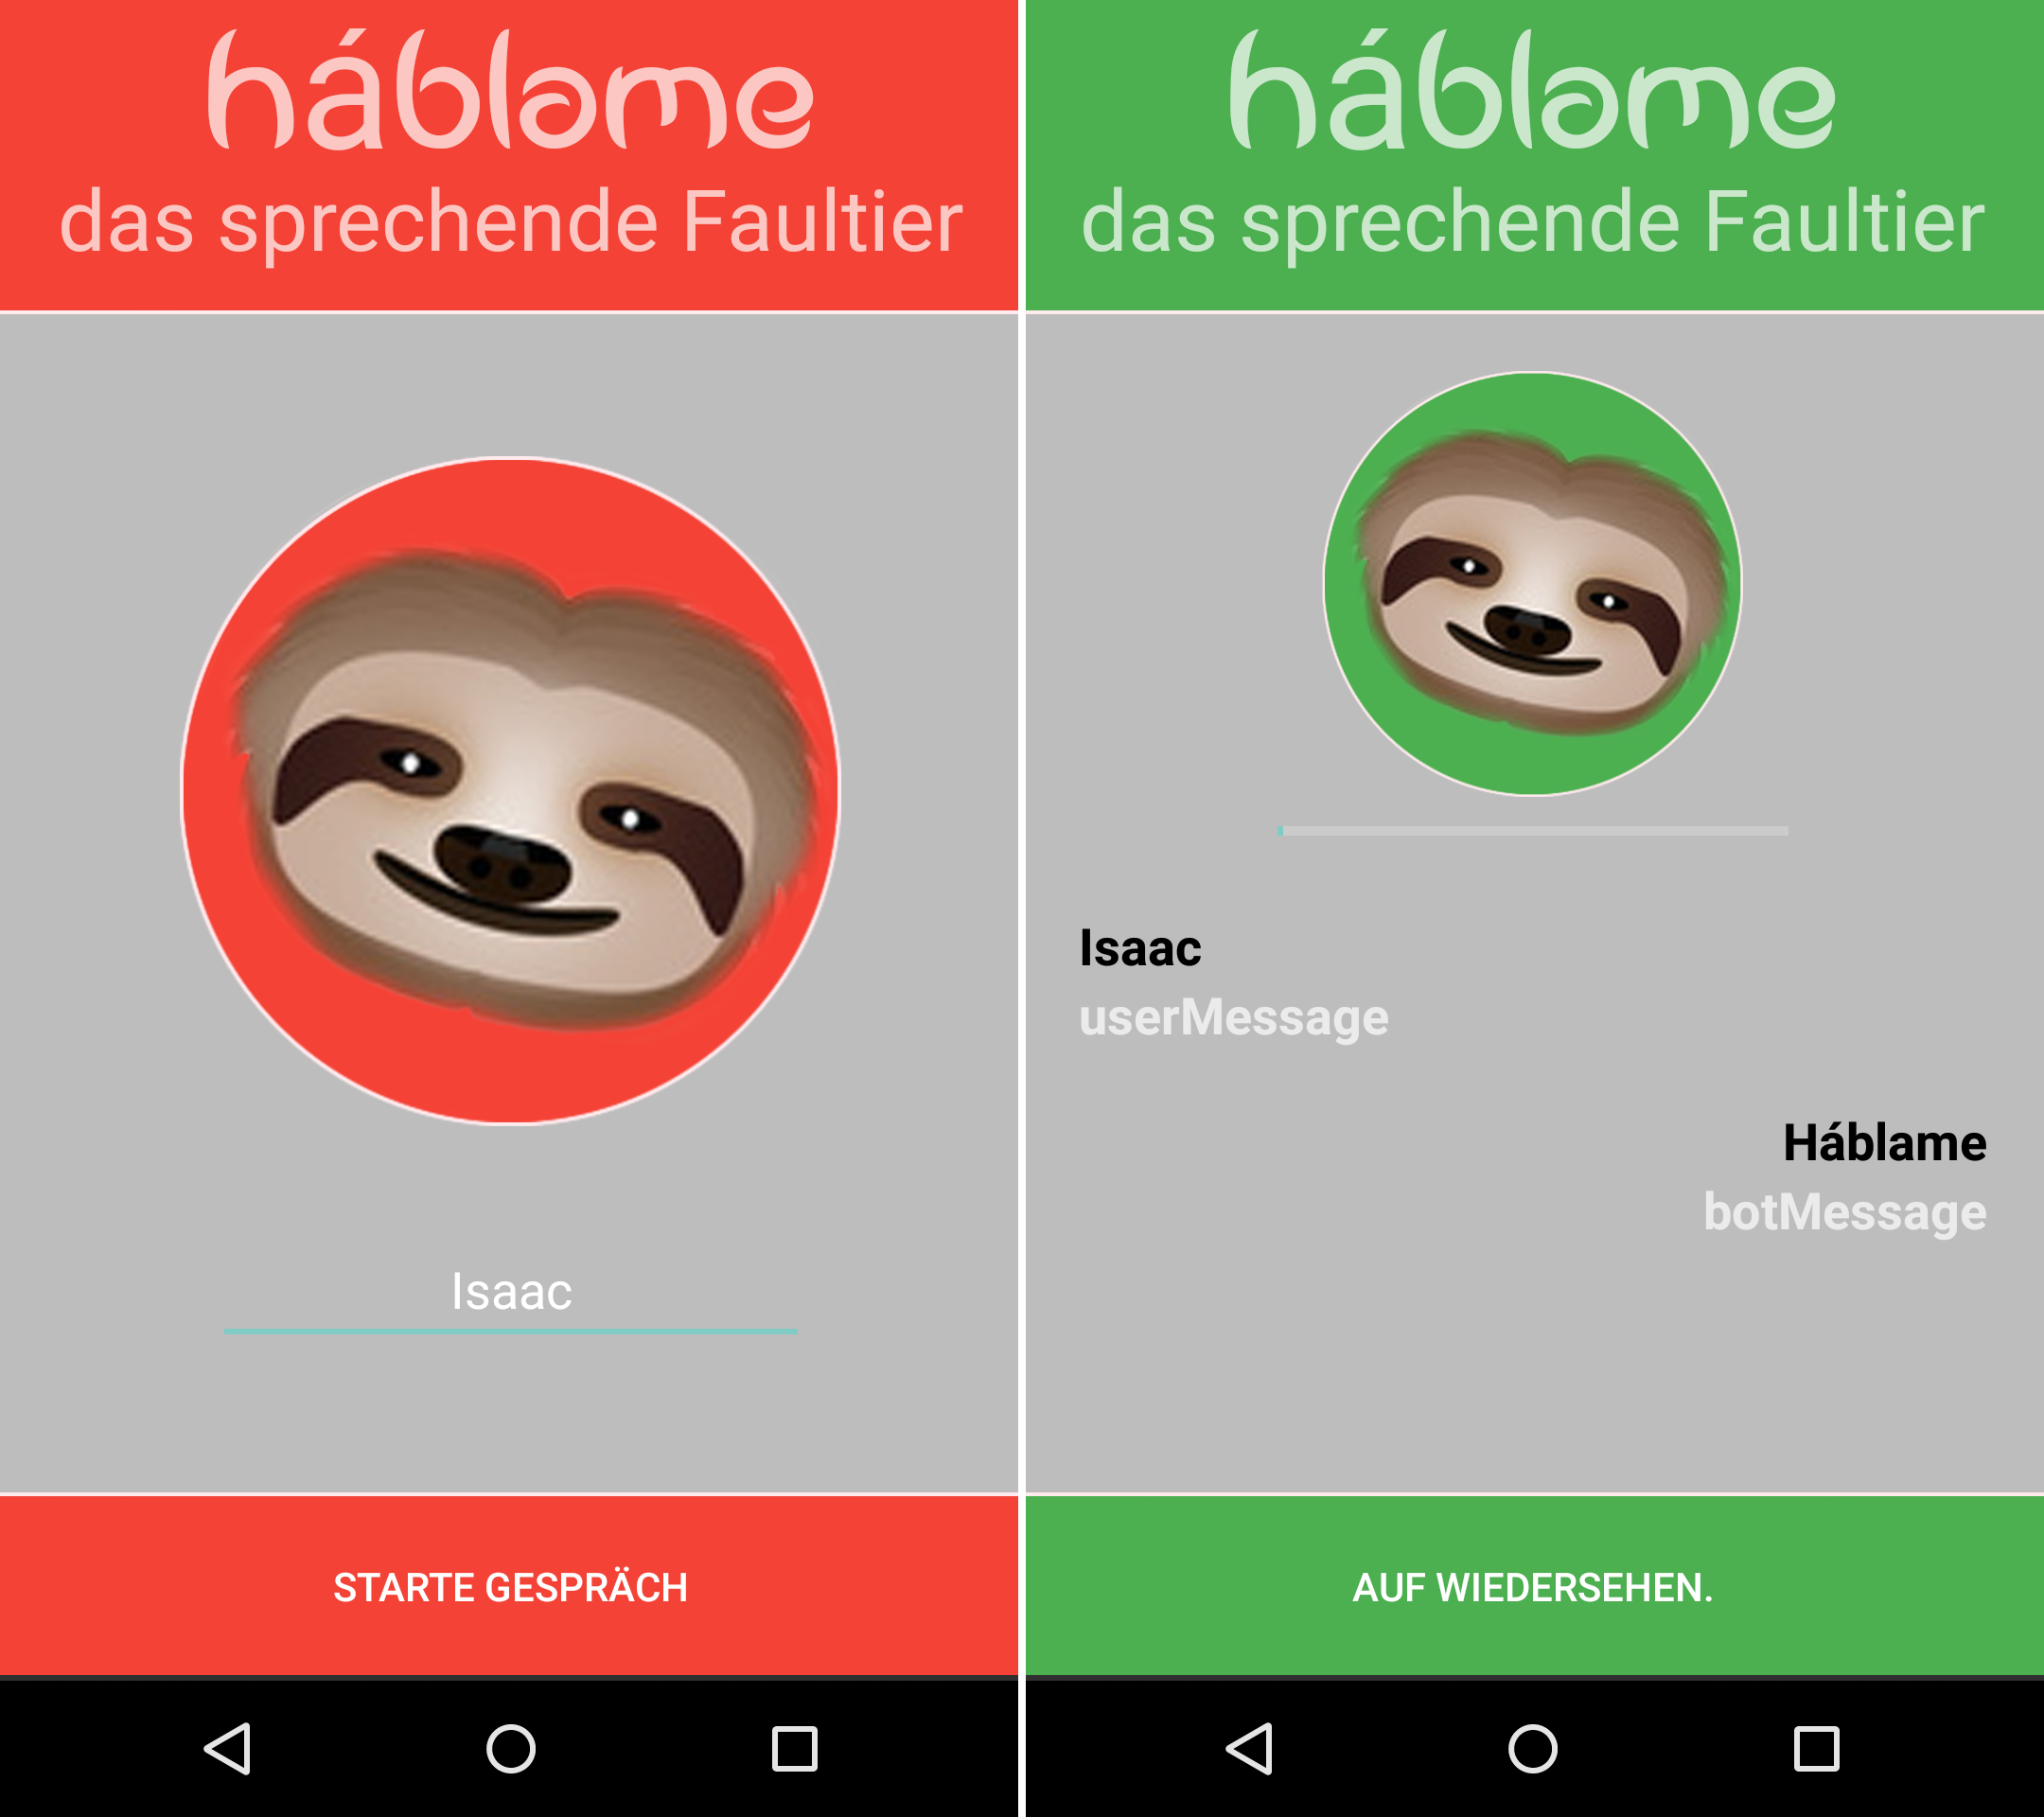
\includegraphics[width=1.0\linewidth]{dh/graphics/hablame-new.png}
		\caption{UI der neuen Android App}
		\label{fig:hablame-new}
	\end{figure}